\graphicspath{ {./figures/} }
\section{Research}
\subsection{Basic Dynamics in Quadrupeds}
\subsection{Kinematics}
 Kinematics is  often referred to as the geometry of motion and describes the motion of points, bodies and systems of bodies without considering the forces that describe the motion. A kinematics problem begins by describing the geometry of the system and declaring the initial conditions of any known values of position, velocity and/or acceleration of points within the system. Then, using arguments from geometry, the position, velocity and acceleration of any unknown parts of the system can be determined. Using kinematics there are a variety of different calculations that can be done to help create an accurate and useful model of a robot. 
    \subsubsection{Forward Kinematics}
    Forward Kinematics refers to the use of kinematic equations to determine the position, usually in x, y, z coordinate space, of an end effector given specific joint parameters with relation to a specific reference point. In the case of a serial manipulator, this is very useful in understanding where the end of the robot will be if given a set of joint values. There are many different ways of calculating forward kinematics, however one of the most universally accepted and used methods is through the use of Denavit–Hartenberg parameters (DH parameters).
    \begin{center}
    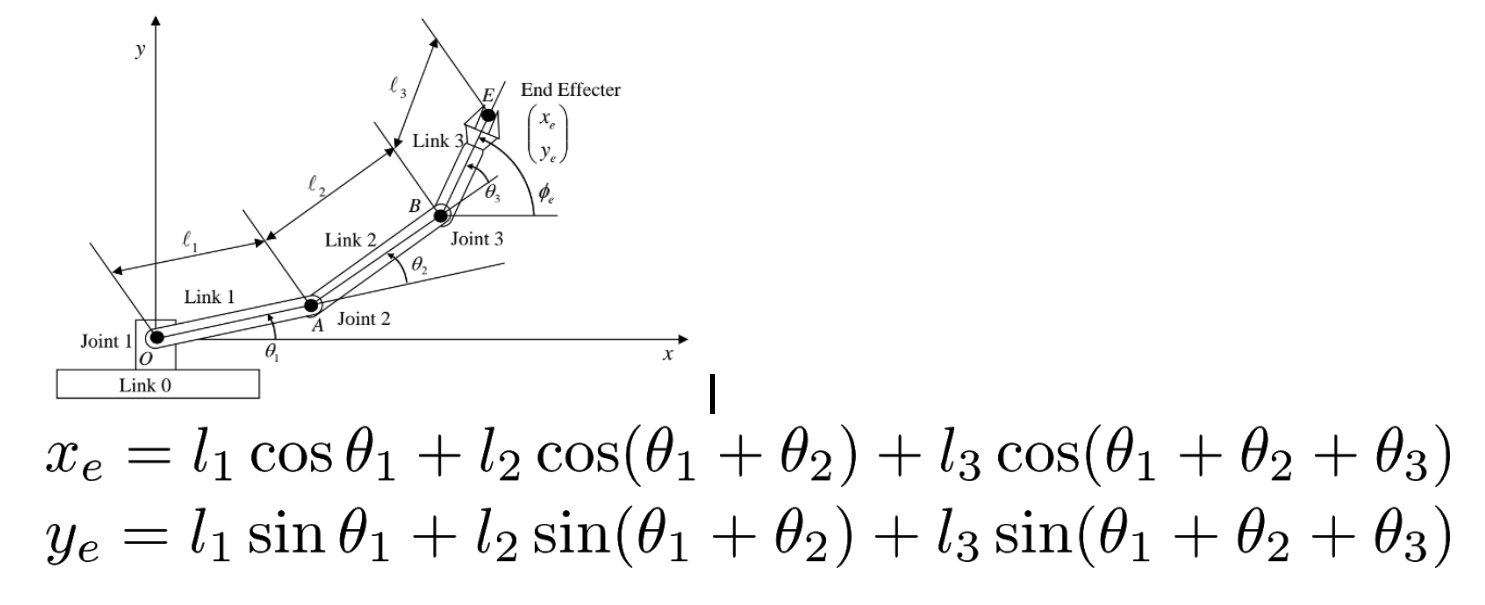
\includegraphics[width=150mm]{3dof.PNG}
    \end{center}
    \subsubsection{DH Parameters}
    In mechanical engineering and robotics, DH parameters are the four parameters associated with a particular convention for attaching reference frames to the links of a spatial kinematic chain, or serial robot manipulator.
    \begin{center}
    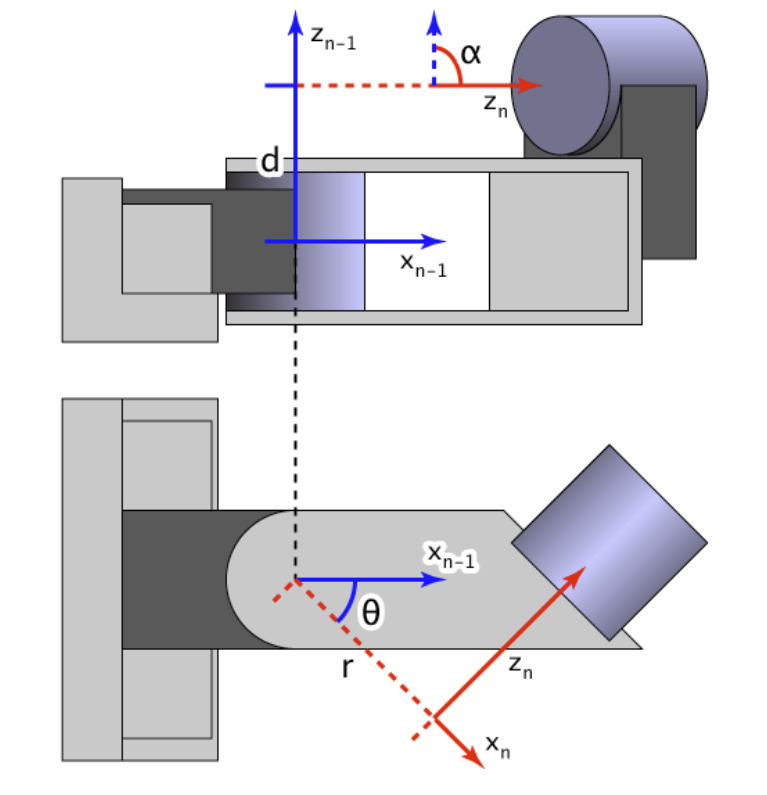
\includegraphics[width=75mm]{Dh.PNG}
    \end{center}
    Coordinate frames are attached to the joints between two links such that one transformation is associated with the joint, [Z], and the second is associated with the link [X]. The coordinate transformations along a serial robot consisting of n links form the kinematics equations of the robot. At its core D-H parameters are coordinate frames attached to the joints between two links such that one transformation is associated with the joint denoted as Z, and the other is associated with the link denoted as X. By multiplying these together you can describe a single link and its joint in a robot manipulator. The coordinate transformations along an entire serial robot consisting of n links form the kinematics equations of the robot.
    \begin{equation}
    [T] = [Z_1][X_1][Z_2][X_2]...[X_{n-1}][Z_n][X_n]

    \end{equation}
    The coordinate transformations [Z] and [X], are determined by modeling the joints connecting the links as either hinged or sliding joints. By doing this, each of the joints can then be further described by a unique line S in space that forms the joint axis and define the relative movement of the two links. A typical serial robot is characterized by a sequence of these lines. For example in a six degree of freedom serial manipulator there are six Si where i = 1,...,6, one for each joint in the robot. For each sequence of lines Si and Si+1, there is a common normal line Ai,i+1. The system of six joint axes Si and five common normal lines Ai,i+1 form the kinematic skeleton of this six degree of freedom serial robot. Denavit and Hartenberg introduced the convention that Z coordinate axes are assigned to the joint axes Si and X coordinate axes are assigned to the common normals Ai,i+1.

    This convention allows the definition of the movement of links around a common joint axis Si by the screw displacement,
    \begin{center}
    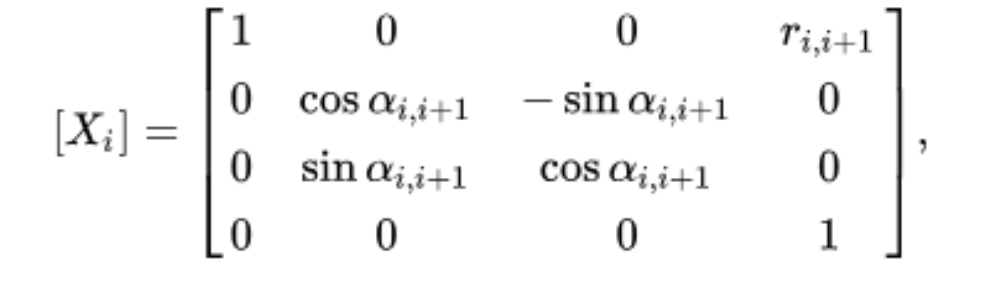
\includegraphics[width=150mm]{xframe.PNG}
    \end{center}
    where θi is the rotation around and di is the slide along the Z axis. Depending on how the robot is constructed either of the parameters θ or d can be constants. The dimensions of each link in the serial chain are defined by the screw displacement around the common normal Ai,i+1 from the joint Si to Si+1, which is given by
    \begin{center}
    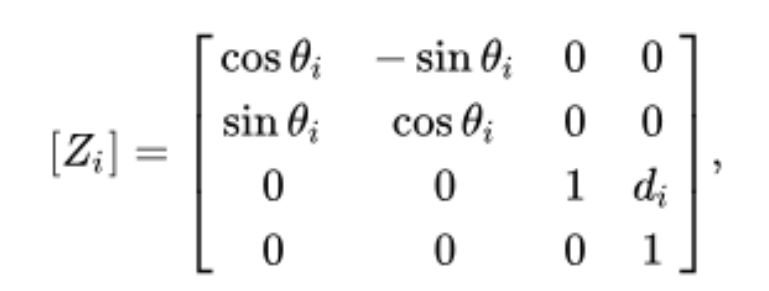
\includegraphics[width=150mm]{zframe.PNG}
    \end{center}
    where αi,i+1 and ri,i+1 define the physical dimensions of the link in terms of the angle measured around and distance measured along the X axis. 
    
    As a rule of thumb, the reference frames should follow the 3 rules below.
    \begin{enumerate}
        \item The Z axis is in the direction of the joint axis
        \item The X axis is parallel to the common normal. If there is no unique common normal or the axes are parallel then d becomes a free parameter.
        \item The Y axis completes the reference frame in accordance to the right-handed coordinate frame system.
    \end{enumerate}
    
    A screw displacement can be separated into the product of its translation and rotation about a line. This also helps better explain how this convention of forward kinematics is describing the position of each joint. By doing this the Z axis transformations can be described as;
    \begin{equation}
    [Z_i] = Trans_{Z_i}(d_i)Rot_{Z_i}(\theta_i)
    \end{equation}
    And the X axis transformations are;
    \begin{equation}
    [X_i] = Trans_{X_i}(r_{i,i+1})Rot_{X_i}(\alpha_{i,i+1})
    \end{equation}
    Using this notation, each link can be described by a coordinate transformation from the concurrent coordinate system to the previous coordinate system simply by multiplying each of these transformations together resulting in;
    \begin{equation}
    ^{n-1}T_n=Trans_{z_{n-1}}(d_n)*Rot_{z_{n-1}}(\theta_n)*Trans_{x_n}(r_n)*Rot_{x_n}(\alpha_n)
    \end{equation}
    Breaking each of these transformations into there matrix transformations we get;
    \begin{center}
    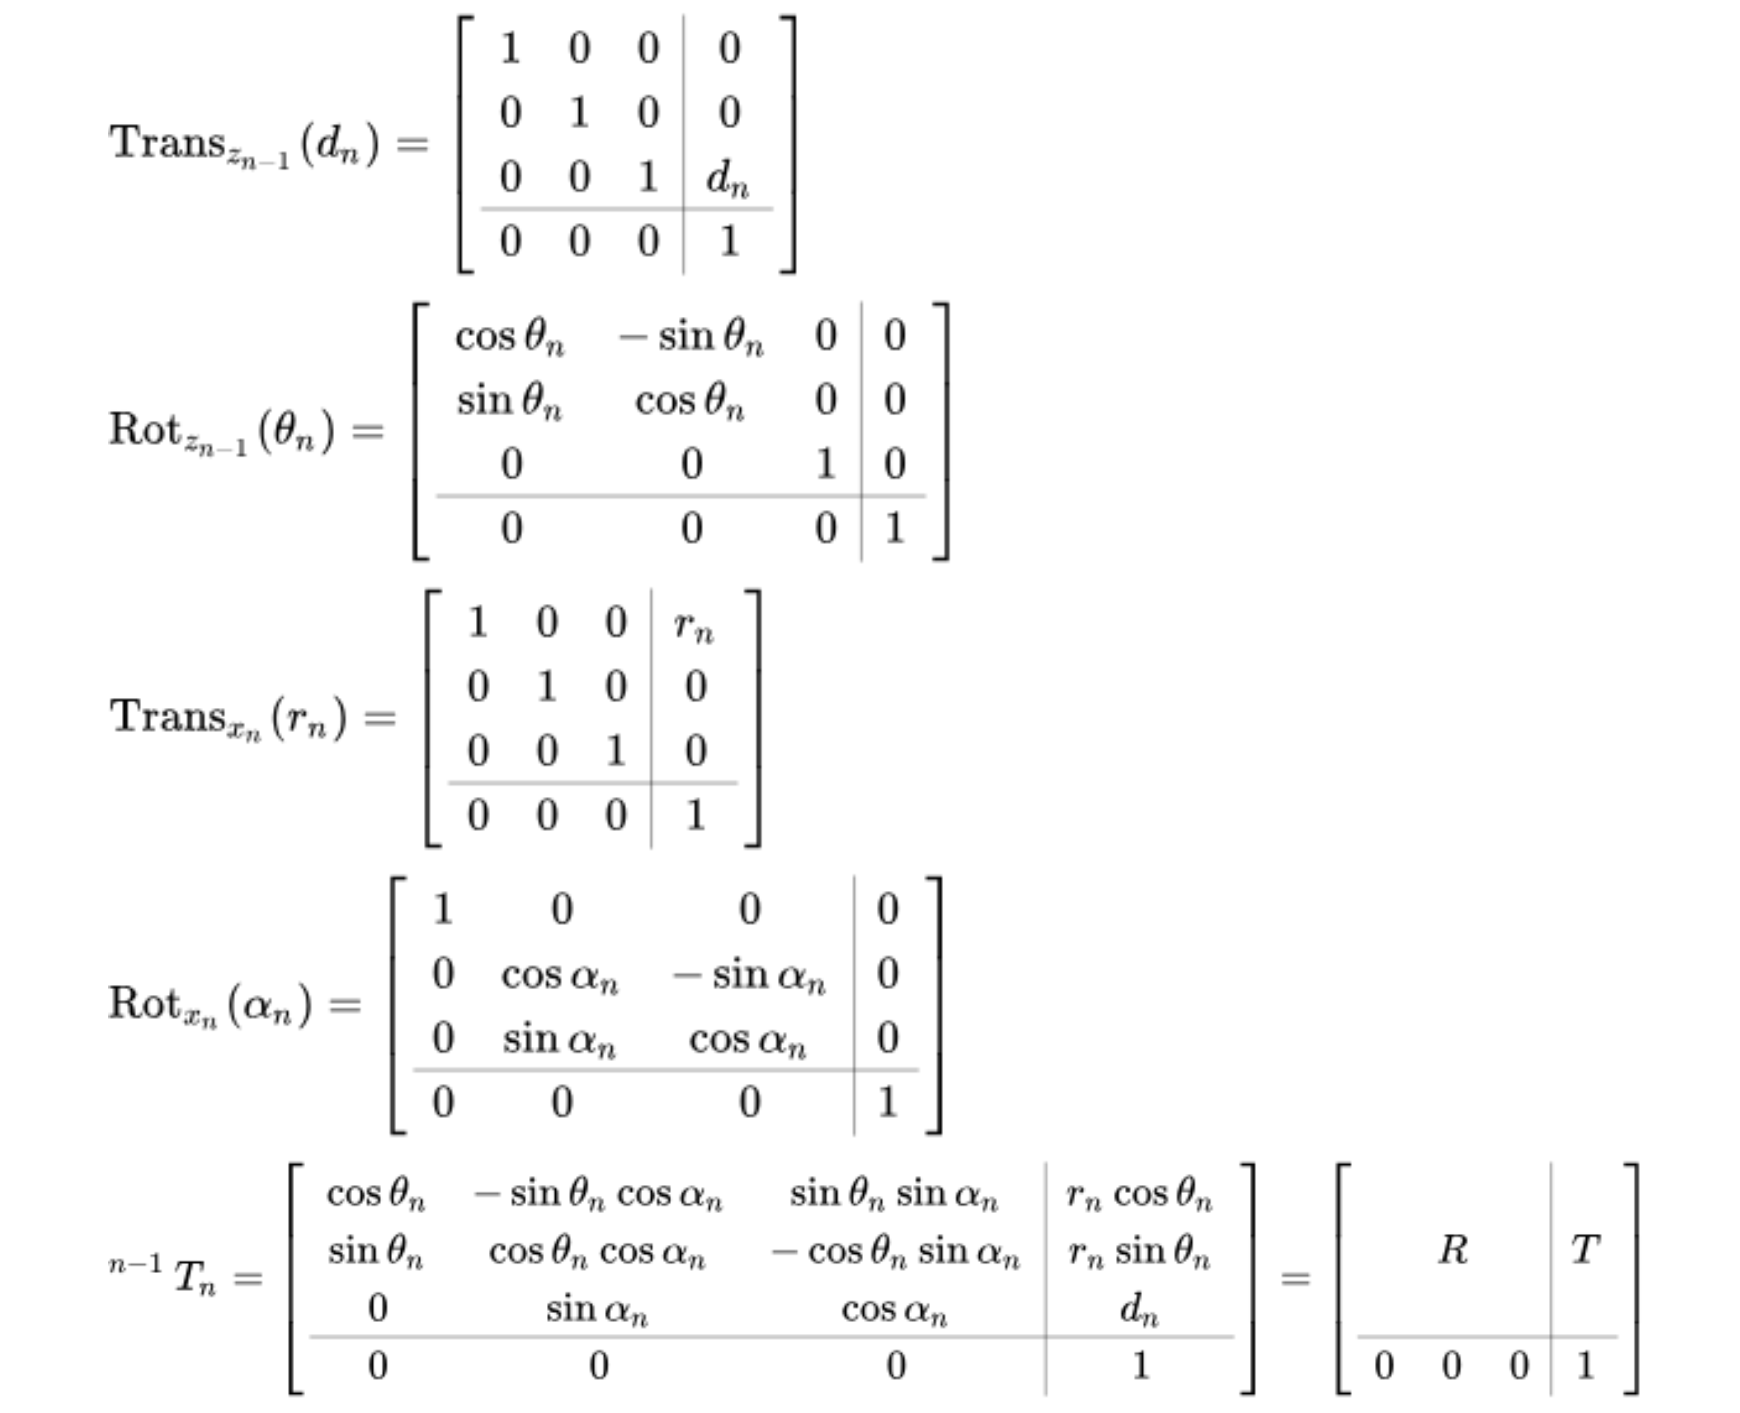
\includegraphics[width=150mm]{Transformation.PNG}
    \end{center}
    At this point we can introduce the actual D-H parameters They were briefly mentioned above when describing the screw displacements but are described below;
    \begin{itemize}
        \item d: offset along previous  z to the common normal
        \item $\theta$: angle about previous z, from old x to new x
        \item r or a: length of the common normal a.. Assuming a revolute joint, this is the radius about previous z.
        \item $\alpha$ angle about common normal, from old z axis to new z axis
    \end{itemize}
    Combining everything we have discussed, the screw displacement, transformation matrix and d-h parameters we get a matrix that looks like the following;
    \begin{center}
    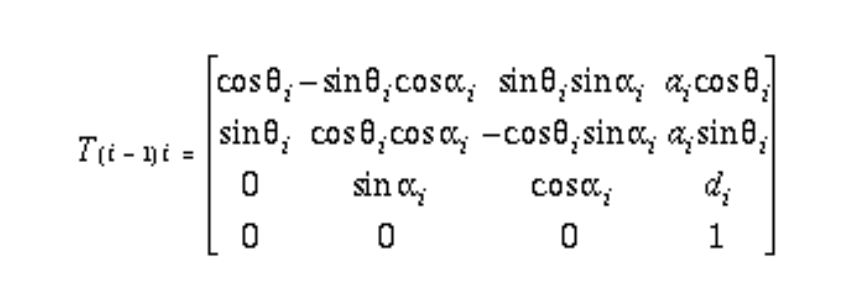
\includegraphics[width=150mm]{Matrizx.PNG}
    \end{center}
    By placing the reference frames using the rules above and using this matrix the forward kinematics of any serial manipulator can be easily determined where the x,y,z of the end effector is described as the 3x1 matrix $[T_x; T_y; T_z]$ in the result of the final matrix; 
     \begin{center}
    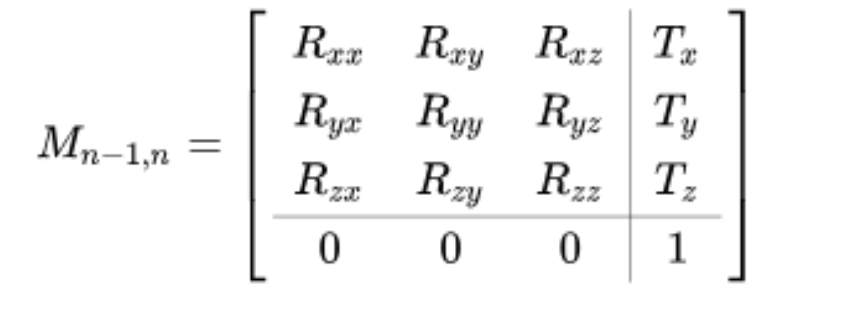
\includegraphics[width=150mm]{Matrix2.PNG}
    \end{center}
    
\subsection{Gaits}
    \subsubsection{What is a gait}
    A gait is the motion of taking  a step. This includes the motion of each joint, the time at each place, the speed of motion and the time between cycles. In the case of a quadruped robot, the 
    
    \subsubsection{Types of gaits}
    




